\section{Mapa i orientacja przestrzenna}
    W celach testowych została napisana dedykowana aplikacja graficzna do sterowani pojazdem oraz reprezentująca mapę użytkownikowi.
    Na zdjęciu \ref{fig:app} przedstawiono interfejs aplikacji.
    \begin{figure}[!ht]
        \centering
        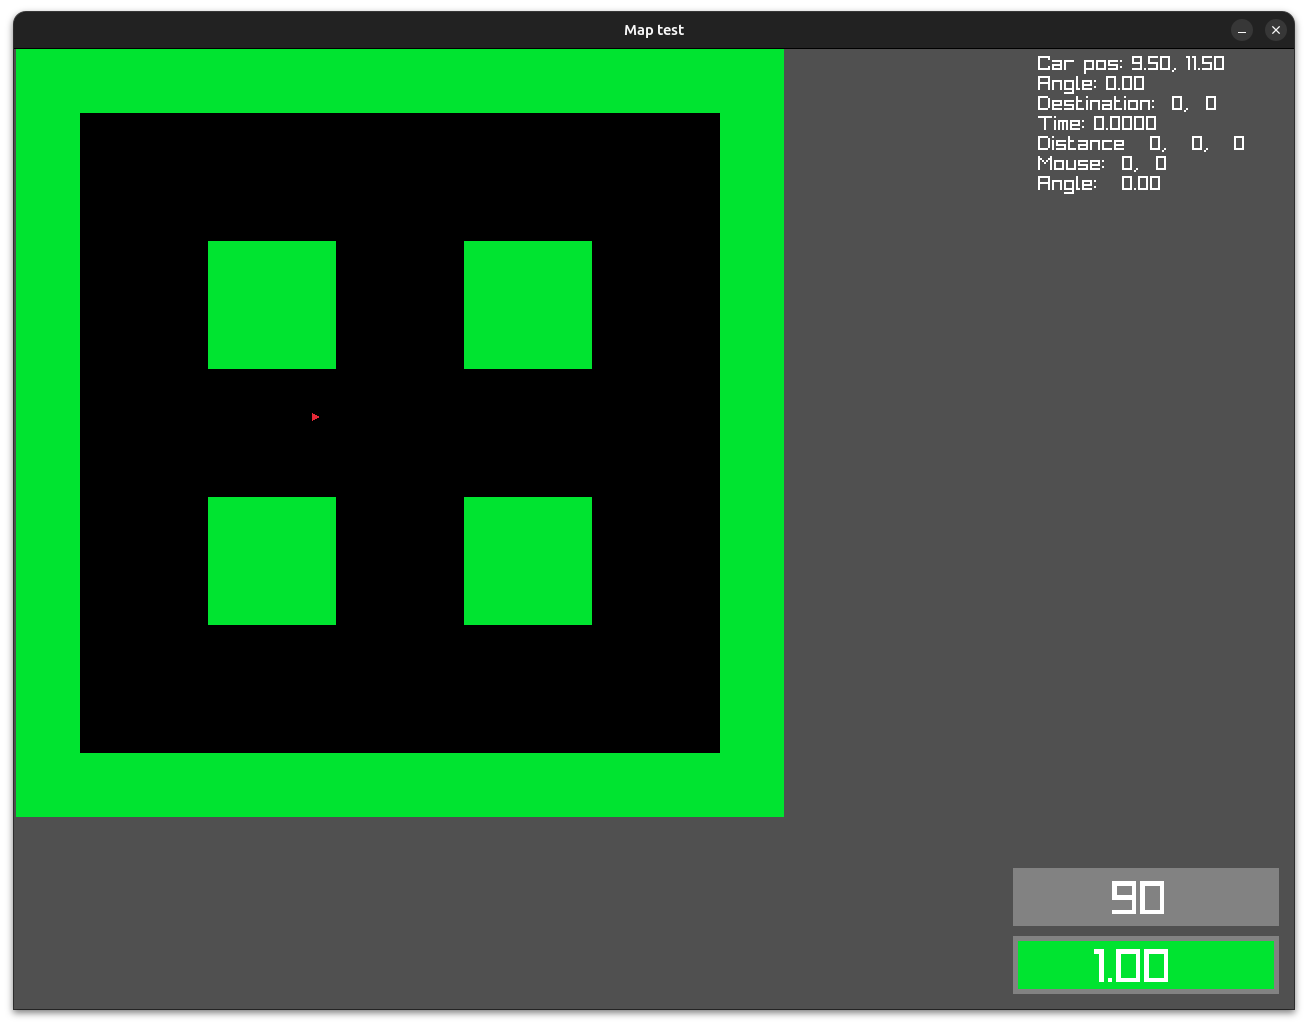
\includegraphics[width = 0.7\textwidth]{PathFinding/App.png}
        \caption{Interfejs aplikacji}
        \label{fig:app}
    \end{figure}
    Interfejs aplikacji składa się z trzech części:
    \begin{enumerate}
        \item Mapa -- reprezentująca aktualnie zbadanego obszar oraz aktualną pozycję pojazdu.
        \item Informacje -- w prawym górnym rogu, wyświetlane są dodatkowe informacje, takie jak aktualna pozycja pojazdu, czy myszy.
        \item Ślizgacze -- w prawym dolnym rogu, znajdują się dwa ślizgacze, górny pozwala precyzyjnie ustawić kąt skrętu kół a dolny pozwala na ustawienie prędkości pojazdu.
    \end{enumerate}

    \subsection{Budowa mapy}
        W założeniu aplikacja ma pozwalać jedynie na wyświetlanie, mapy zbudowanej przez samochód.
        Natomiast wszystkie obliczenia powinny zostać wykonane przez kontroler zarządzający pojazdem.
        Jednak ze względu na duże skomplikowanie opisywanych problemów w celach testowych, to aplikacja posiada zaimplementowany algorytm do wyszukiwania ścieżek.
        Następnie wyznaczona ścieżka zamieniana jest na proste instrukcje w stylu ,,uruchom oba silniki na 500mm'' czy ,,skręć kołami o $30^\circ$ w lewo''.




    \subsection{Wyznaczanie ścieżek}
        Kliknięcie na mapę, pozwala na wybranie punktu docelowego, do które zostanie wyznaczona ścieżka, po której pojazd będzie się poruszał.
        Dzięki zastosowaniu algorytmu Dijkstry opisanego w rozdziale \ref{subsec:algorytm_odnajdowania_ścieżek}, możliwe jest wyznaczcie optymalnej ścieżki.
        Następnie wyznaczona ścieżka zamieniana jest na instrukcje ruchu.

        \subsubsection{Algorytm odnajdowania ścieżek}
        \label{subsec:algorytm_odnajdowania_ścieżek}
            Wyznaczanie optymalnej ścieżki, od wielu lat jest bardzo popularnym problemem w informatyce i robotyce.
            Istnieje wiele artykułów, skupiających się na tej tematyce, a także wiele gotowych rozwiązań.
            Najpopularniejszymi algorytmami są:
            \begin{itemize}
                \item algorytm A* (A star),
                \item algorytm Dijkstry,
                \item algorytm Bellmana-Forda.
            \end{itemize}

            Poniżej przedstawione zostaną wyniki pracy \citetitle{AnalizaAlgorytmówŚcieżek} \cite{AnalizaAlgorytmówŚcieżek}
            autorstwa: Beata \citeauthor{AnalizaAlgorytmówŚcieżek}.
            \begin{figure}[!ht]
                \centering
                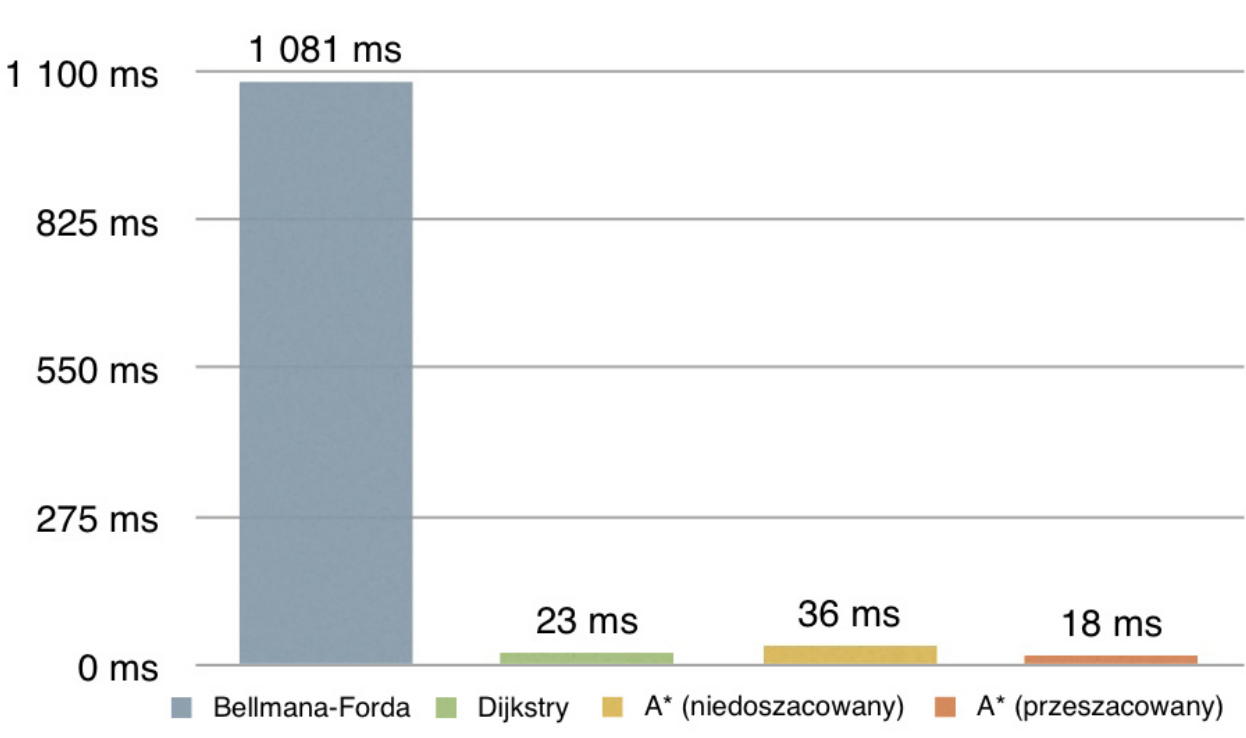
\includegraphics[width=0.7\textwidth]{PathFinding/Wykres_sredni_czas_algorytmu_pathfinding.png}
                \caption{Wykres porównania średniego czasu wykonania algorytmów}
                Źródło:\cite{AnalizaAlgorytmówŚcieżek} \citetitle{AnalizaAlgorytmówŚcieżek}
                \label{fig:PathFindingTime}
            \end{figure}
            \begin{figure}[!ht]
                \centering
                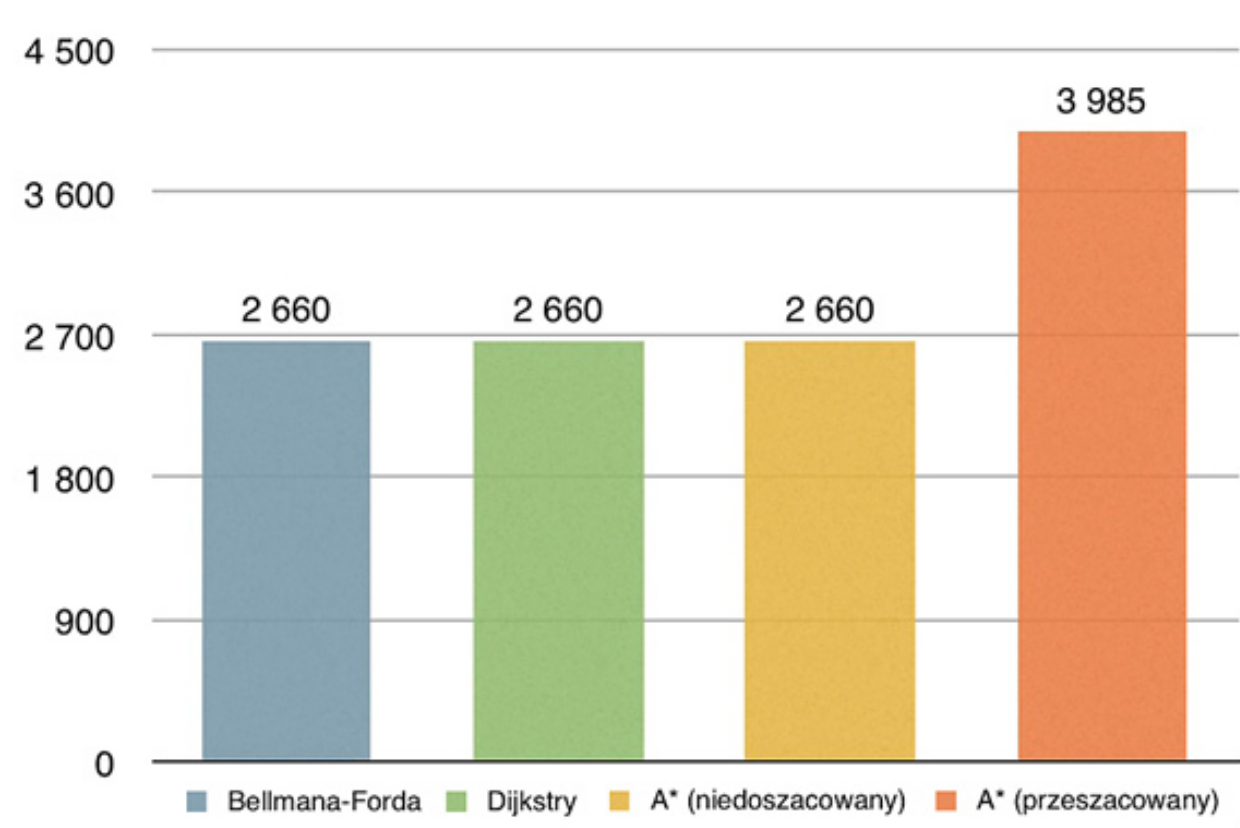
\includegraphics[width=0.7\textwidth]{PathFinding/Wykres_sredni_koszt_algorytmu_pathfinding.png}
                \caption{Wykres porównania średniego kosztu znalezionych ścieżek}
                Źródło:\cite{AnalizaAlgorytmówŚcieżek} \citetitle{AnalizaAlgorytmówŚcieżek}
                \label{fig:PathFindingCost}
            \end{figure}

            Z powyższej pracy wynika, że najlepszym rozwiązaniem jest algorytm Dijkstry.
            Dodatkowym czynnikiem potwierdzającą powyższe stwierdzenie jest samo skomplikowanie algorytmu.
            Algorytm Dijkstry jest stosunkowo prosty w implementacji, a także posiada niski koszt obliczeniowy.
            Dzięki czemu wydaje się najlepszym rozwiązaniem dla zastosowań w układach embedded.


% \newpage
            \subsection{Wygładzanie ścieżek}
            \label{subsec:wygładzanie_ścieżek}
            Na rysunku \ref{fig:pathfinding_dikstra} przedstawiono przykładową ścieżkę wyznaczoną przez algorytm Dijkstry.
            Algorytm ten zwraca najkrótsze możliwe połączenie między dwoma punkami.
            Najczęściej jest to prosta łącząca dwa punkty.
            Jednak ze względu na ograniczenia kontrakcyjne wyrysowana trasa jest niemożliwa do wykonania przez drona.

            \begin{figure}[!ht]
                \centering
                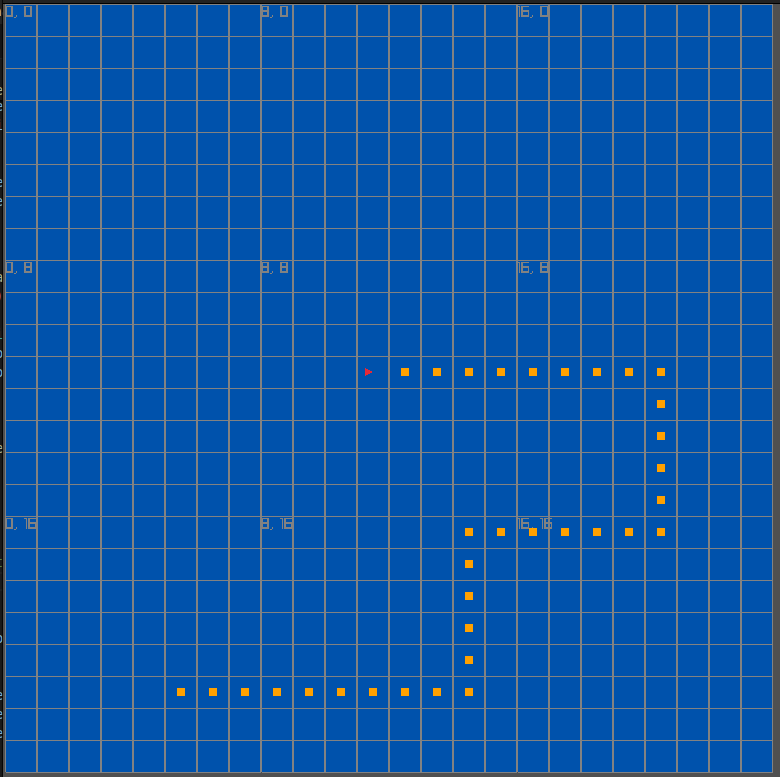
\includegraphics[width = 0.7\textwidth, trim = {120px, 30px, 20px, 300px}, clip]{PathFinding/pathfinding_dikstra.png}
                \caption{Przykładowa ścieżka wyznaczona przez algorytm Dijkstry}
                \label{fig:pathfinding_dikstra}
            \end{figure}

% \newpage
            Budowany pojazd ma tylko jedną oś skrętną, więc nie jest w stanie skręcić w miejscu.
            Dlatego koniecznym jest zastosowanie algorytmu wygładzania trasy.
            W artykule \citetitle{Simple_PathSmoothing} \cite{Simple_PathSmoothing}, przedstawiona jest najprostsza możliwa metoda wygładzania.
            Przedstawiony algorytm zakłada zbudowanie mapy punktów o nie całkowitych współrzędnych.
            Dzięki czemu możliwe jest przesunięcie punktów docelowych z środka pojedynczej kratki w kierunku łuku skrętu.

            \begin{figure}[!ht]
                \centering
                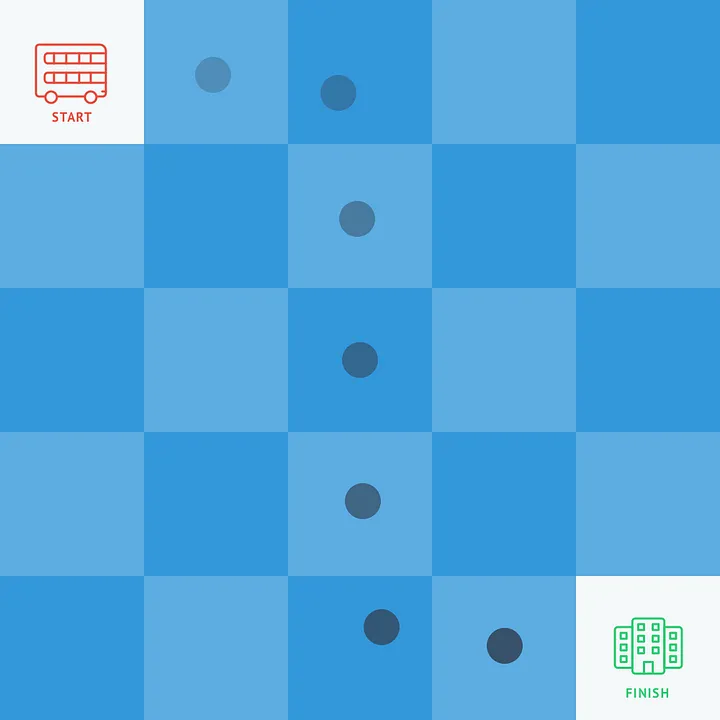
\includegraphics[width = 0.5\textwidth]{PathFinding/simple_pathSmooth.jpeg}
                \caption{Przykład wygładzania ścieżki na podstawie artykułu}
                \citetitle{Simple_PathSmoothing} \cite{Simple_PathSmoothing}
                \label{fig:simple_pathSmooth}
            \end{figure}

            Zaletą przedstawionego rozwiązania jest niewątpliwie jego prostota.
            Jednak olbrzymią wadą    jest brak kontroli nad wygładzeniem trasy, a także pocięcie drogi na pojedyncze punkty między którymi pojazd będzie stawał i ponownie ruszał.
            Dodatkowo, pojawia się problem przechowywania mapy w pamięci (problem ten został dokładniej opisany w rozdziale \ref{subsec:przechowywanie_mapy}).
            W związku z powyższym autor zdecydował się na zastosowanie bardziej skomplikowanego algorytmu.

            Alternatywne metody wygładzenia ścieżek zostały opisane w artykułach: \citetitle{Compare_PathSmoothing} \cite{Compare_PathSmoothing} oraz \citetitle{Compare_PathSmoothing2} \cite{Compare_PathSmoothing2}.
            Oba artykuły przedstawiają i porównują różne metody dostosowywania wyznaczonej ścieżki do możliwości robota.
            Poniżej na wykresie \ref{fig:smoothingPath_res}
            \begin{figure}[!ht]
                \centering
                \begin{minipage}{0.49\textwidth}
                    \centering
                    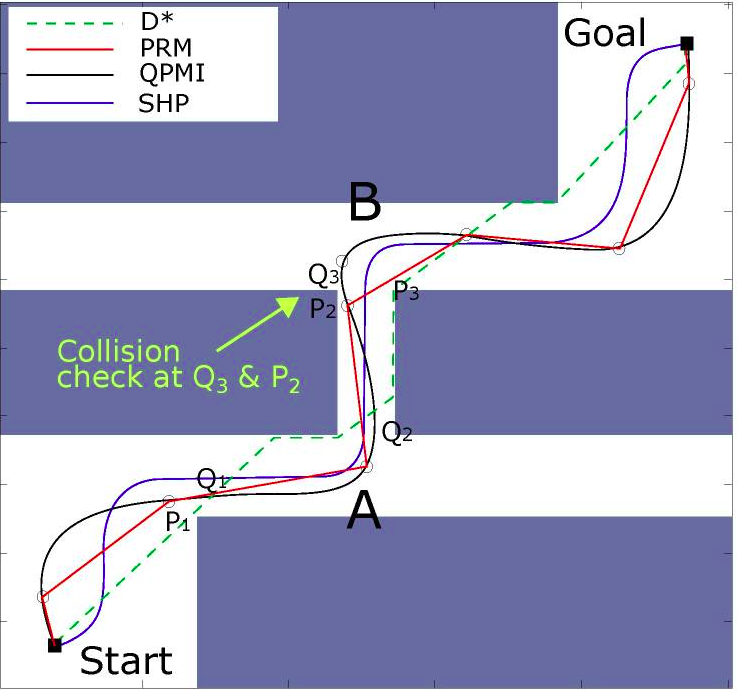
\includegraphics[width = \textwidth]{PathFinding/smoothingPath.png}
                    Źródło: \cite{Compare_PathSmoothing}
                \end{minipage}
                \begin{minipage}{0.49\textwidth}
                    \centering
                    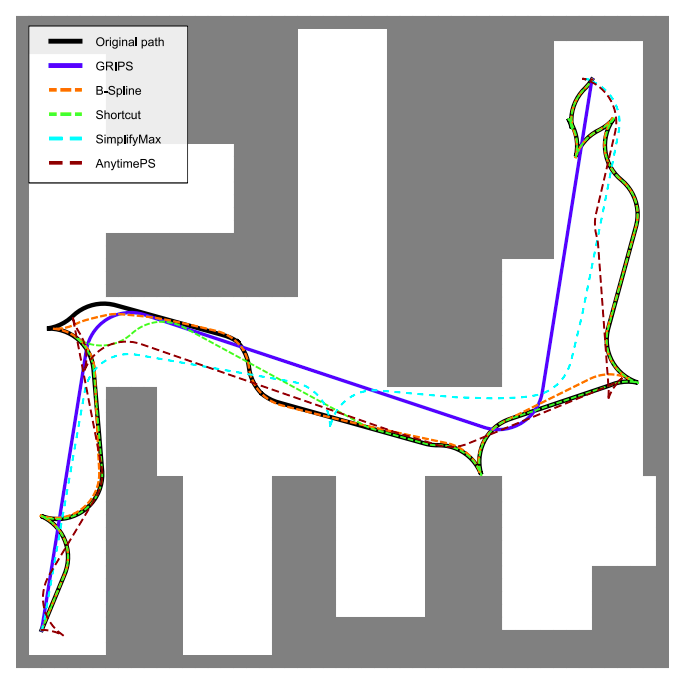
\includegraphics[width = \textwidth]{PathFinding/smoothingPath2.png}
                    Źródło: \cite{Compare_PathSmoothing2}
                \end{minipage}
                \caption{Przedstawienie tras wygładzonych przez różne algorytmy}
                \label{fig:smoothingPath_res}
            \end{figure}

            Ostatecznie ze wszystkich wymienionych w artykułach algorytmów został wybrany algorytm krzywych Dublina - ze względu na łatwą implementację oraz możliwość łatwego dostosowywania promienia skrętu.

% \newpage
            \subsubsection{Opis algorytmu krzywych Dublina}
                Mechanizm wygładzania ścieżek za pomocą krzywych Dublina jest przeznaczony dla pojazdów o ograniczonej sterowności.
                Przykładowo dla pojazdów z tylko jedną osią skrętną.
                \begin{figure}[!ht]
                    \centering
                    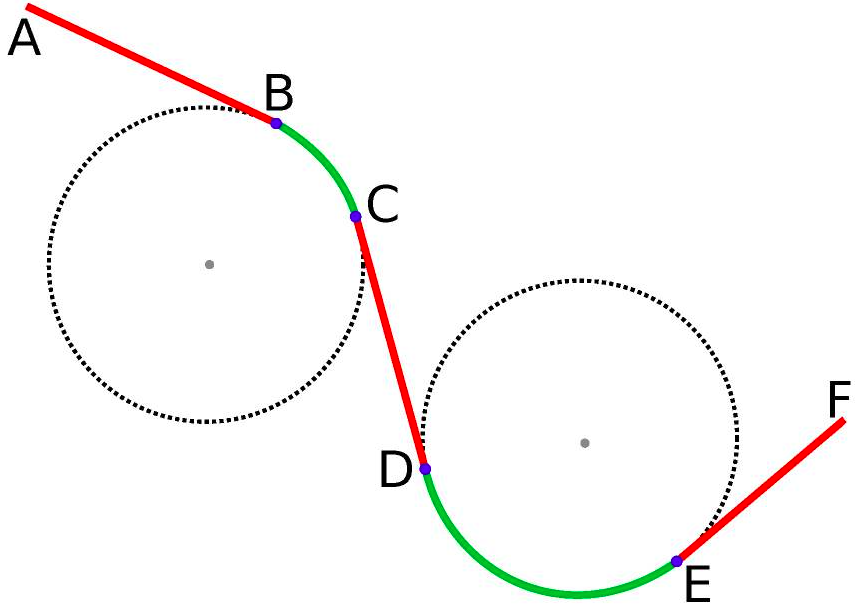
\includegraphics[width = 0.375\textwidth]{PathFinding/dublinCurves.png}
                    \caption{Schemat ścieżki z kołami o minimalnych promieniach}
                    \label{fig:dublinCurves}
                    Źródło: \citetitle{Compare_PathSmoothing}\cite{Compare_PathSmoothing}
                \end{figure}

            \begin{wrapfigure}[3]{R}{0.3\textwidth}
                \centering
                \vspace{1cm}
                \begin{tikzpicture}
                    \draw
                        (0,  0.0) node[draw, circle, minimum width = 0.5cm, align=center](A){1}
                        (0, -1.5) node[draw, circle, minimum width = 0.5cm, align=center](B){2}
                        (0, -3.0) node[draw, circle, minimum width = 0.5cm, align=center](C){3}
                        (0, -4.5) node[draw, circle, minimum width = 0.5cm, align=center](D){4}
                        (0, -6.0) node[draw, circle, minimum width = 0.5cm, align=center](E){5}
                        (0, -7.5) node[draw, circle, minimum width = 0.5cm, align=center](F){6}
                    ;
                    \draw[-Stealth] (A) -- (B);
                    \draw[-Stealth] (B) -- (C);
                    \draw[-Stealth] (C) -- (D);
                    \draw[-Stealth] (D) -- (E);
                    \draw[-Stealth] (E) -- (F);
                    \draw[-Stealth] (F) to[bend right] (A);

                \end{tikzpicture}
            \end{wrapfigure}

\newpage
            Poniżej przedstawiono implementację algorytmu krzywych Dublina zastosowanego w projekcie.
            Przedstawiony wersja jest z założenie nieoptymalną modyfikacją oryginału.

            \vspace{0.25cm}
            \begin{minipage}[l]{0.6\textwidth}
                \begin{enumerate}
                    \item Zamiana punktów ścieżki na listę prostych o punktach początkowych i końcowych.
                    \item Wyznaczenie punku przecięcia się dwóch kolejnych prostych.
                    \item Wyznaczenie dwusiecznej kąta tworzonego przez obie proste w punkcie przecięcia.
                    \item Wyznaczenie kierunku, w którym będzie poruszał się pojazd po zakręcie.
                    \item Znalezienie na dwusiecznej środka okręgu. Punkt ten zawsze znajduje się w przeciwnym kierunku do ruchu pojazdu.
                    \item Znalezienie punktów styczności okręgu i obu prostych. Te punkty będą punktem początkowym i końcowym łuku, po którym porusza się pojazd.
                \end{enumerate}
            \end{minipage}
            \vspace{0.25cm}

            Pierwotne założenia zakładają, że nie należy łączyć dwóch prostych, a zawsze jeśli jest to możliwe ścieżka powinna zaczynać się i kończyć łukiem.
            Jednak w tym projekcie dużo łatwiej jest wyznaczyć łuk łączący dwie proste, niż próbować na siłę wyznaczyć łuk do dowolnego punktu.

            \begin{figure}[!ht]
                \centering
                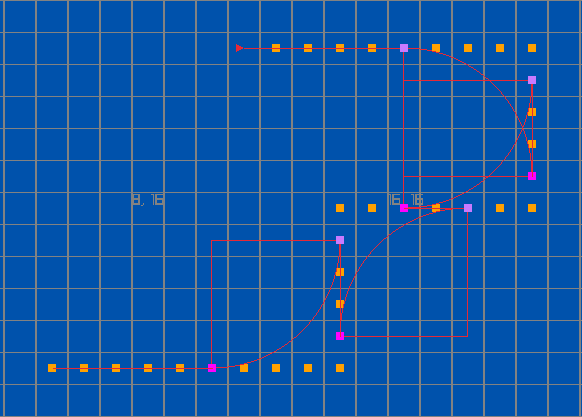
\includegraphics[width = 0.7\textwidth]{PathFinding/path_dublinCurve.png}
                \caption{Wyznaczenie trasy z podziałem na instrukcje}
                \label{fig:path_dublin}
            \end{figure}



    \subsection{Przechowywanie mapy}
    \label{subsec:przechowywanie_mapy}
        Przechowywanie mapy jest niezwykle złożonym zagadnieniem.
        W zależności od zastosowania oraz platformy, na której pracujemy, ta sama mapa może być przedstawiona na różne sposoby.
        Mapa zapisana na komputerze -- o bardzo dużej dostępnej pamięci może być bardzo dokładna.
        Natomiast ta sama mapa zapisana na mikrokontrolerze o bardzo ograniczonej pamięci musi zawierać uproszczenia.

        \subsubsection{Mapa jako tablica ścian}
            W wielu projektach mapę przedstawia się jako tablicę dwuwymiarową, w której poszczególne komórki odpowiadają poszczególnym polom w labiryncie.
            Każda komórka zawiera informacje, w którym kierunku od niej można się poruszać.
            Przykład takiego przechowywania labiryntu przedstawia artykuł \citetitle{maze_storage}\cite{maze_storage}.
            Na rysunku \ref{fig:mazeCellStorage} przedstawione jest proponowane rozwiązanie.

            \begin{figure}[!ht]
                \centering
                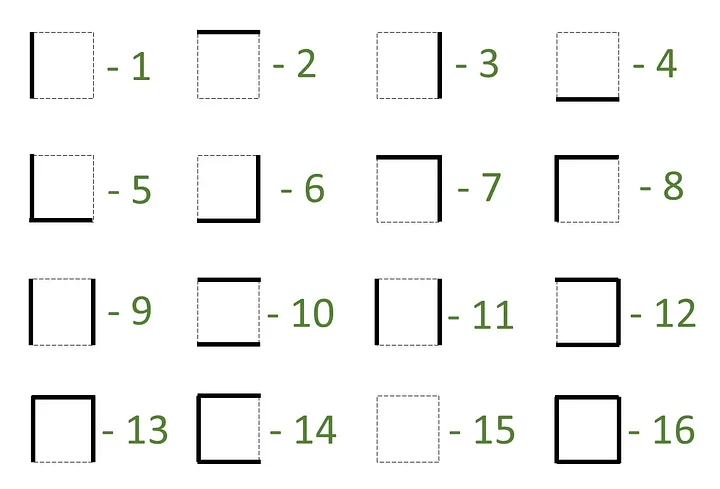
\includegraphics[width = 0.7\textwidth]{mazeCellStorage.jpeg}
                \caption{Przechowywanie komórek labiryntu z informacją o możliwości ruchu}
                Źródło: \citetitle{maze_storage}\cite{maze_storage}
                \label{fig:mazeCellStorage}
            \end{figure}

            Metoda ta jest bardzo skuteczna kiedy znane są dokładne wymiary każdej komórki labirynty.
            Jednak przechowywanie mapy otwartej przestrzeni w taki sposób jest bardzo nieefektywne.
            Przykładowo jeśli z komórki $A$, nie możemy jechać prosto to może oznaczać zarówno, że w miejscu komórki $B$ jest ściana, jak i to, że komórka $B$ jest nie przejezdna.
            W labiryncie gdzie znaczenie mają ściany to rozwiązanie jest bardzo dobre, jednak jeśli nie jesteśmy w stanie powiedzieć czy to co wykrywamy to cienka ścianka czy też duża przeszkoda to rozwiązanie staje się nie optymalne.

            \begin{figure}[!ht]
                \centering
                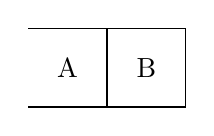
\begin{tikzpicture}
                    \draw
                        (0, 0) -- (1, 0) -- (1, 1) -- (0, 1)
                        (0.5, 0.5) node{A}
                        (1, 0) rectangle (2, 1)
                        (1.5, 0.5) node[]{B}
                    ;
                \end{tikzpicture}
                \caption{Przykład niejednoznaczności wymiarów}
            \end{figure}

            Dodatkowymi wadami przedstawionego rozwiązani są: rozmiar każdej komórki oraz czas potrzebny na przeanalizowanie wszystkich możliwości.
            Pojedynczy kwadrat w powyższej metodzie składa się z 4 bitów dodatkowo łącząc poszczególne kratki ze sobą, okazuje się, że niektóre bity są nadmiarowe.
            Jeśli z punktu $A$ nie możemy jechać do góry, to znaczy że z punktu $C$ nie będzie można jechać w dół.
            Jednak ta informacji musi zostać zapisana dla każdej komórki osobno.
            \begin{figure}[!ht]
                \centering
                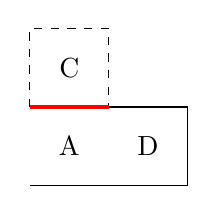
\begin{tikzpicture}
                    \draw
                        (0, 0) -- (1, 0)
                        (1, 0) -- (2, 0) -- (2, 1) -- (1, 1)

                        (0.5, 0.5) node{A}
                        (0.5, 1.5) node{C}
                        (1.5, 0.5) node{D}
                    ;
                    \draw[dashed]
                        (0, 1) rectangle (1, 2)
                    ;
                    \draw[ultra thick, red]
                        (0, 1) -- (1, 1)
                    ;
                \end{tikzpicture}
                \caption{Przykład nadmiarowych informacji}
            \end{figure}\\
            Analogiczna sytuacja występuje kiedy trasa jest przejedza (tak jak dla połączenia między~$A$~i~$D$).

            Podsumowując, powyższa metoda przechowywania mapy nadaje się jedynie do labiryntów, o jasno określonych zasadach.
            To rozwiązanie nie sprawdzi się do reprezentacji otwartej przestrzeni.
            Posiada za dużo wad, aby można było próbować ją zastosować w rzeczywistości.

        \subsubsection{Mapy wektorowe}
            Innym podejściem do przedstawionego problemu jest zastosowanie wektorów.
            W takim przypadku nie rozważamy terenu jako pojedyncze komórki, a proste figure geometryczne.
            Takie podejście zostało opisane w artykule \citetitle{vector_map}\cite{vector_map}.
            Na zdjęciu \ref{fig:buildVectMap} przedstawiono algorytm budowania takiej mapy.

            \begin{figure}[!ht]
                \centering
                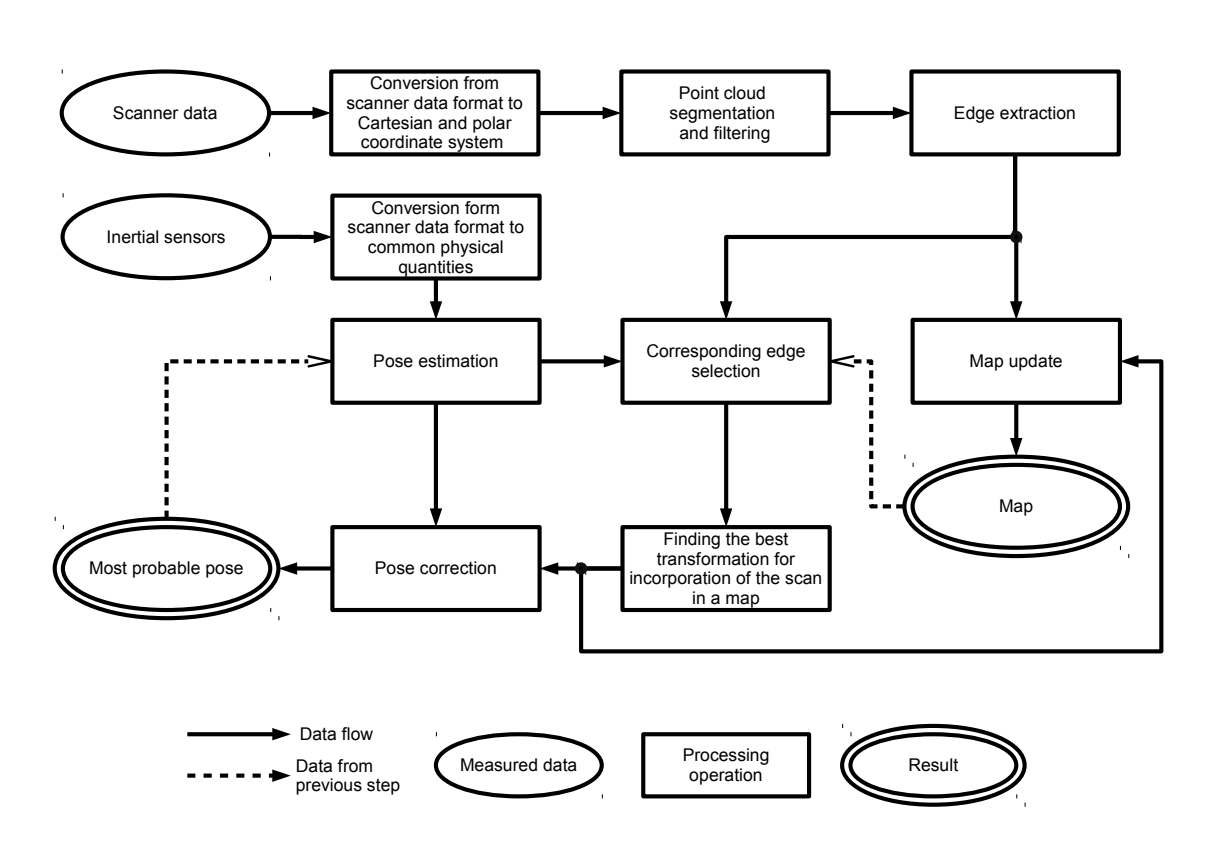
\includegraphics[width = \textwidth]{VectMapAlogirthm.png}
                \caption{Ogólny schemat przetwarzania punktów w mapę wektorową}
                Źródło: \citetitle{vector_map}\cite{vector_map}
                \label{fig:buildVectMap}
            \end{figure}

            Jak widać przedstawiony na powyższym rysunku (rys. \ref{fig:buildMap}) algorytm nie należy do prostych.
            Wymaga on bardzo dokładnego procesu pomiarowego, który nie ogranicza się tylko do minimalnej ilości punktów.
            A najlepsze efekty daje dla pełnego skanu otoczenia.

            Przedstawiona metoda potrzebuje zarówno nadmiarowości - nowy obszar musi w jakimś stopniu pokrywać się z wcześniej zbadanym,
            to również obliczenie nowego położenia oraz połączenie poszczególnych punktów w wektory wymaga dużo czasu.
            Co więcej wyznaczanie trasy w tak skomplikowanej mapie trwa bardzo długo.
            Na schemacie \ref{schematic:vectorMapPathfinding} przedstawiono algorytm sprawdzania kolizji na trasie dla mapy wektorowej.

            \begin{figure}[!ht]
    \centering
    \begin{tikzpicture}
        \draw[]
            (0,  0) node[draw, circle, minimum width = 2cm, align = center](start){Nowa\\ścieżki}
            (-3, -2.5) node[draw, circle, minimum width = 2cm, align = center](instruction){Ścieżka na\\instrukcje}
            (0, -6) node[draw, diamond, minimum width = 2cm, align = center](check){Czy występuje\\kolizja}
            (6, -6) node[minimum width = 2cm, align = center](noCollision){Powtarzaj dla wszystkich\\instrukcji i wektorów}
        ;

        \draw[-Stealth] (start) to[bend left] (instruction);
        \draw[-Stealth] (instruction) to[bend right] (check);
        \draw[-Stealth] (check) to[bend right] node[right]{Tak} (start);
        \draw (check) to[bend right] node[below]{Nie} (noCollision);
        \draw[-Stealth] (noCollision) to[bend right] (check);
    \end{tikzpicture}
    \caption{Uproszczony algorytm do wyznaczania ścieżek na mapie wektorowej}
    \label{schematic:vectorMapPathfinding}
\end{figure}

            Natomiast olbrzymimi zaletami takiego rozwiązania jest możliwość olbrzymiego skalowania - w przeciwieństwie do map rastrowych nie występuje zjawisko ,,pixelizacji''.
            Jak również mały rozmiar takiej mapy oraz możliwość bardzo dokładnego wyznaczania trasy.


\newpage
        \subsubsection{Mapa rastrowa}
            Ostatnim przedstawionym rozwiązaniem jest mapa rastrowa.
            W tym przypadku dzielimy całą przestrzeń na równe kwadraty, a każdy z kwadratów opisuje jeden z kilku możliwych stanów.
            Przykładowe stany to:
            \begin{enumerate}
                \item pole nieznane,
                \item pole wolne,
                \item pole zajęte.
            \end{enumerate}

            Olbrzymią wadą tej metody jest dyskretyzacja przestrzeni, która w zależności od rozmiaru pojedynczej komórki może za bardzo przekłamywać rzeczywistość.
            Przykładowo dla komórek o rozmiarze $100mm \times 100mm$, obiekty o mniejszych wymiarach, mogą być albo całkowicie niewidoczne, albo zajmować całą komórkę.
            Dlatego niezwykle ważne jest aby dostosować wymiary pojedynczej kratki, zarówno do wymiarów pojazdu, jak i wymiarów całej przestrzeni.

            Następnym problemem jest duża ilość pamięci potrzebna do przechowywania takiej mapy.
            Przykładowo: dla mapy o wymiarach $10m \times 10m$ i pojedynczych komórkach o rozmiarze $100mm \times 100mm$ daje rozmiar:
            \begin{gather}
                V_{\text{size}} = \frac{10m}{100mm} \cdot \frac{10m}{100mm} \cdot 2bit = 20kbit
            \end{gather}

            Taką mapę należało również optymalnie rozłożyć w pamięci, tak aby możliwy był szybki dostęp do całej grupy komórek.
            Przykładowo dla mapy przechowywanej na mikrokontrolerze, nie istotne jest czy pole jest nieznane czy wolne - w obu przypadkach algorytm do wyznaczanie ścieżek zachowa się tak samo.
            Dlatego można ograniczyć ilość bitów na kratkę do jednego.
            Dodatkowo możemy ułożyć poszczególne komórki w zbiory odpowiadające większym kwadratom.
            I tak:
            \begin{itemize}[label = -]
                \item osiem komórek w rzędzie to jeden bajt,
                \item osiem rzędów to jeden wiersz, a więc osiem bajtów,
            \end{itemize}
            dzięki czemu dostęp do całego wiersza jest bardzo szybki.
            Jednocześnie procesor nie musi za każdym razem zwracać się o dostęp do pamięci, jeśli chce odczytać informacje o następnej komórce.

            Ze względu na swoją prostote i łatwość implementacji to właśnie ten sposób przechowywania mapy został zastosowany w projekcie.
            Dlatego też sposobu dla komputera został policzony średni czas potrzebny na wyznaczenie ścieżki na trasie testowej przedstawionej na zdjęciu \ref{fig:pathFindingTime}.
            \begin{figure}
                \centering
                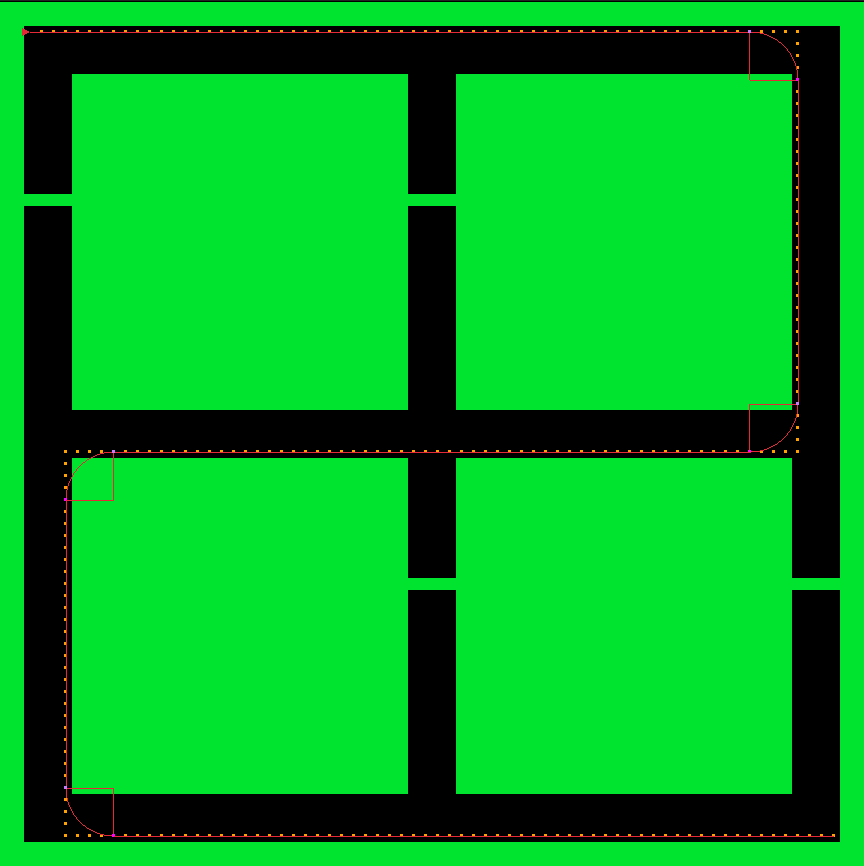
\includegraphics[width=0.6\textwidth]{TestMap.png}
                \caption{Pomiar czasu wyznaczania ścieżki}
                Wymiary mapy: 72 komórki na 72 komórki
                \label{fig:pathFindingTime}
            \end{figure}

            Średni czas potrzebny na wyznaczenie ścieżki wynosił około $100ms$.
            Złożoność mapy ma niewielki wpływ na czas wyznaczenia ścieżek.
            Dla pustej mapy czas ten oscylował wokół $95ms$.
            Pozycja pojazdu oraz odległość do celu także mają nieznaczący wpływ na czas wyznaczenie trasy.

    \subsection{Nanoszenie punktów pomiarowych}
        Jednym z podstawowych założeń była możliwość budowania mapy przez pojazd.
        W tym celu samochód musi mierzyć odległość w trakcie ruchu.
        Czujniki ToF zamontowane na przedzie pojazdu zostały ustawione w tryb ciągłego pomiaru odległości z okresem pomiarowym $T ms$.
        Takie ustawienie pozwala na regularne odczytywanie odległości bez konieczności zajmowani procesora procedurą pomiarową.

        \subsection{Czas pomiarowy}
            Czas odebrania pomiaru od pojedynczego czujnika wynosi około $3ms$.
            Dlatego okres pomiarowy powinien być na tyle długi, aby pozwolić na odczytanie wszystkich czujników.
            Wartość $T$ powinna być większa od $9ms$.
            Okres pomiarowy został ustawiony na $T = 100ms$.
            Dzięki czemu pojazd jest w stanie, w miarę na bieżąco, reagować na zdarzenia.

        \subsection{Przykładowa mapa}
            Regularny pomiar oraz znajomość przebytej drogi między każdym z odcinków pozwala na dokładne określenie, w którym miejscu zostały wykonane poszczególne pomiary.
            Poniżej przedstawiono zrzut ekranu (rys. \ref{fig:buildMap}) z aplikacji z początkiem budowanej mapy o wymiarach $ 2.4m \times 2.4m$ i rozmiarze pojedynczej kratki $100mm \times 100mm$.

            \begin{figure}[!ht]
                \centering
                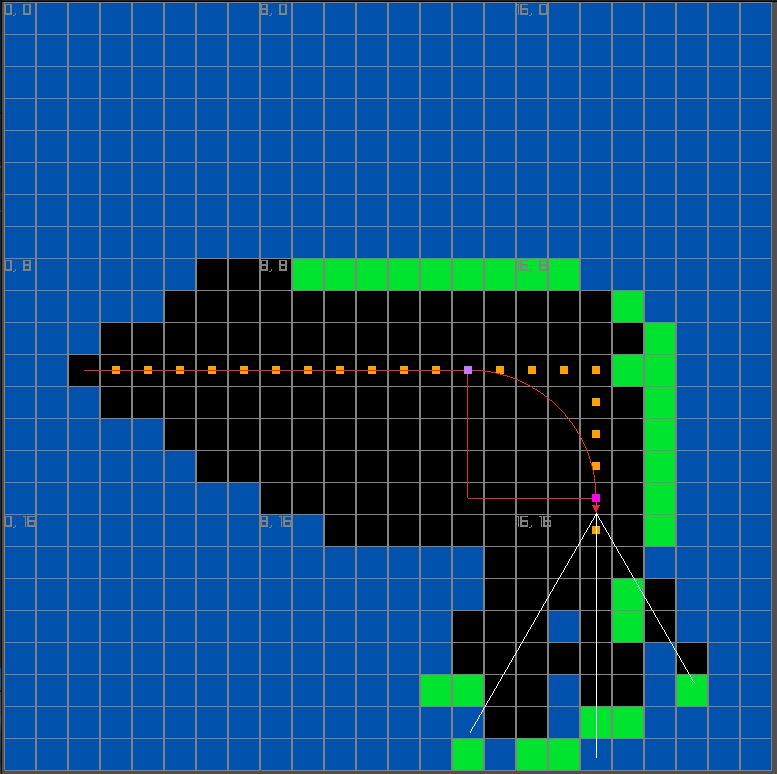
\includegraphics[width=0.6\textwidth]{PathFinding/buildMap.png}
                \caption{Zbudowana mapa}
                \label{fig:buildMap}
            \end{figure}

            \begin{figure}
    \centering
    \begin{tikzpicture}[scale = 2]
        \draw
            (0, 0) rectangle (4.1, 2.7)
            (2, 1.7) --++ (2.1, 0)
            (2, 1.7) --++ (0, 1)
            (3.1, 0.2) --++(1, 0)
            (3.1, 0.2) --++(0,-0.2)
            
            (2.0, 1.5) node[draw, circle, minimum width = 0.5cm, fill = red]{}
            (3.1, 1.5) node[draw, circle, minimum width = 0.5cm, fill = red]{}
            (3.5, 1.0) node[draw, circle, minimum width = 0.5cm, fill = red]{}
        ;
        \draw[color=gray, dashed]
            (2.0, 1.5) -- (3.1, 1.5)
            (3.1, 1.5) arc(90:0:0.4)
        ;

        \draw[Stealth-Stealth] (2, 2) --node[above]{$2.0m$}++ (2.1, 0);
        \draw[Stealth-Stealth] (4.2, 1.7) --node[right]{$1.5m$}++ (0, -1.5);
        \draw[Stealth-Stealth] (3.1,-0.1) --node[below]{$1.0m$}++ (1, 0);
        \draw[Stealth-Stealth] (3.0, 0.2) --node[left]{$0.2m$}++ (0,-0.2);

    \end{tikzpicture}
    \caption{Schemat mapowanego pomieszczenia}
    \label{schematic:room}
\end{figure}

            Na schematycznym rysunku \ref{schematic:room} przedstawiono rzut powierzchni, po której pojazd.
            Na czerwono zaznaczono przybliżone miejsca zatrzymania się pojazdu, a linią przerywaną pokazuje pokonaną trasę.
            Jak widać odzwierciedlenie mapy, stworzonej przez drona, jest dość dokładne względem rzeczywistego terenu.

            Widać pewne zniekształcenia wynikające prawdopodobnie z niskiej rodzielczości mapy oraz nie idealność algorytmu rysującego.
            Pomimo tego przedstawioną próbę można uznać za udaną.